%%==================================================
%% chapter02.tex for NWPU Bachelor Thesis
%% Encoding: UTF-8
%%==================================================

\chapter{设计}
\label{chap:Design}
本章将具体描述FAT32文件系统接口的整体架构和设计思路。
从要求实现的功能出发,将本接口分为两个模块,并为每个模块都设计符合规定的应用程序接口(API)以供上层程序调用。
本章仅在逻辑层面进行工程的设计描述,具体的算法实现将在第\ref{chap:Implementation}章详述。

\section{架构设计}
\label{sec:Architecture}
通过分层的模块化设计,将整个文件接口要求达成的功能全部通过上层模块的预留API体现出来,这样,顶层的用户应用程序也无需关心底层的驱动和硬件。
分层如下:
\begin{enumerate}[noitemsep,topsep=0pt,parsep=0pt,partopsep=0pt]
    \item
FAT文件系统模块,主要是FAT32文件系统的设计,包括识别并挂载FAT32文件系统、创建并打开文件、在文件中读取数据和写入数据、修改数据等功能,
控制着数据在磁盘卷的具体组织形式,在逻辑上负责了磁盘和内存的数据交互。
    \item
SD卡驱动模块,主要是SD卡相关函数功能的设计,包括SD卡初始化进入SPI模式、读写扇区数据等功能,是联系整个软件层与硬件层的桥梁,控制着数据的物理传输。
\end{enumerate}

\begin{figure}[!htb]
    \centering
    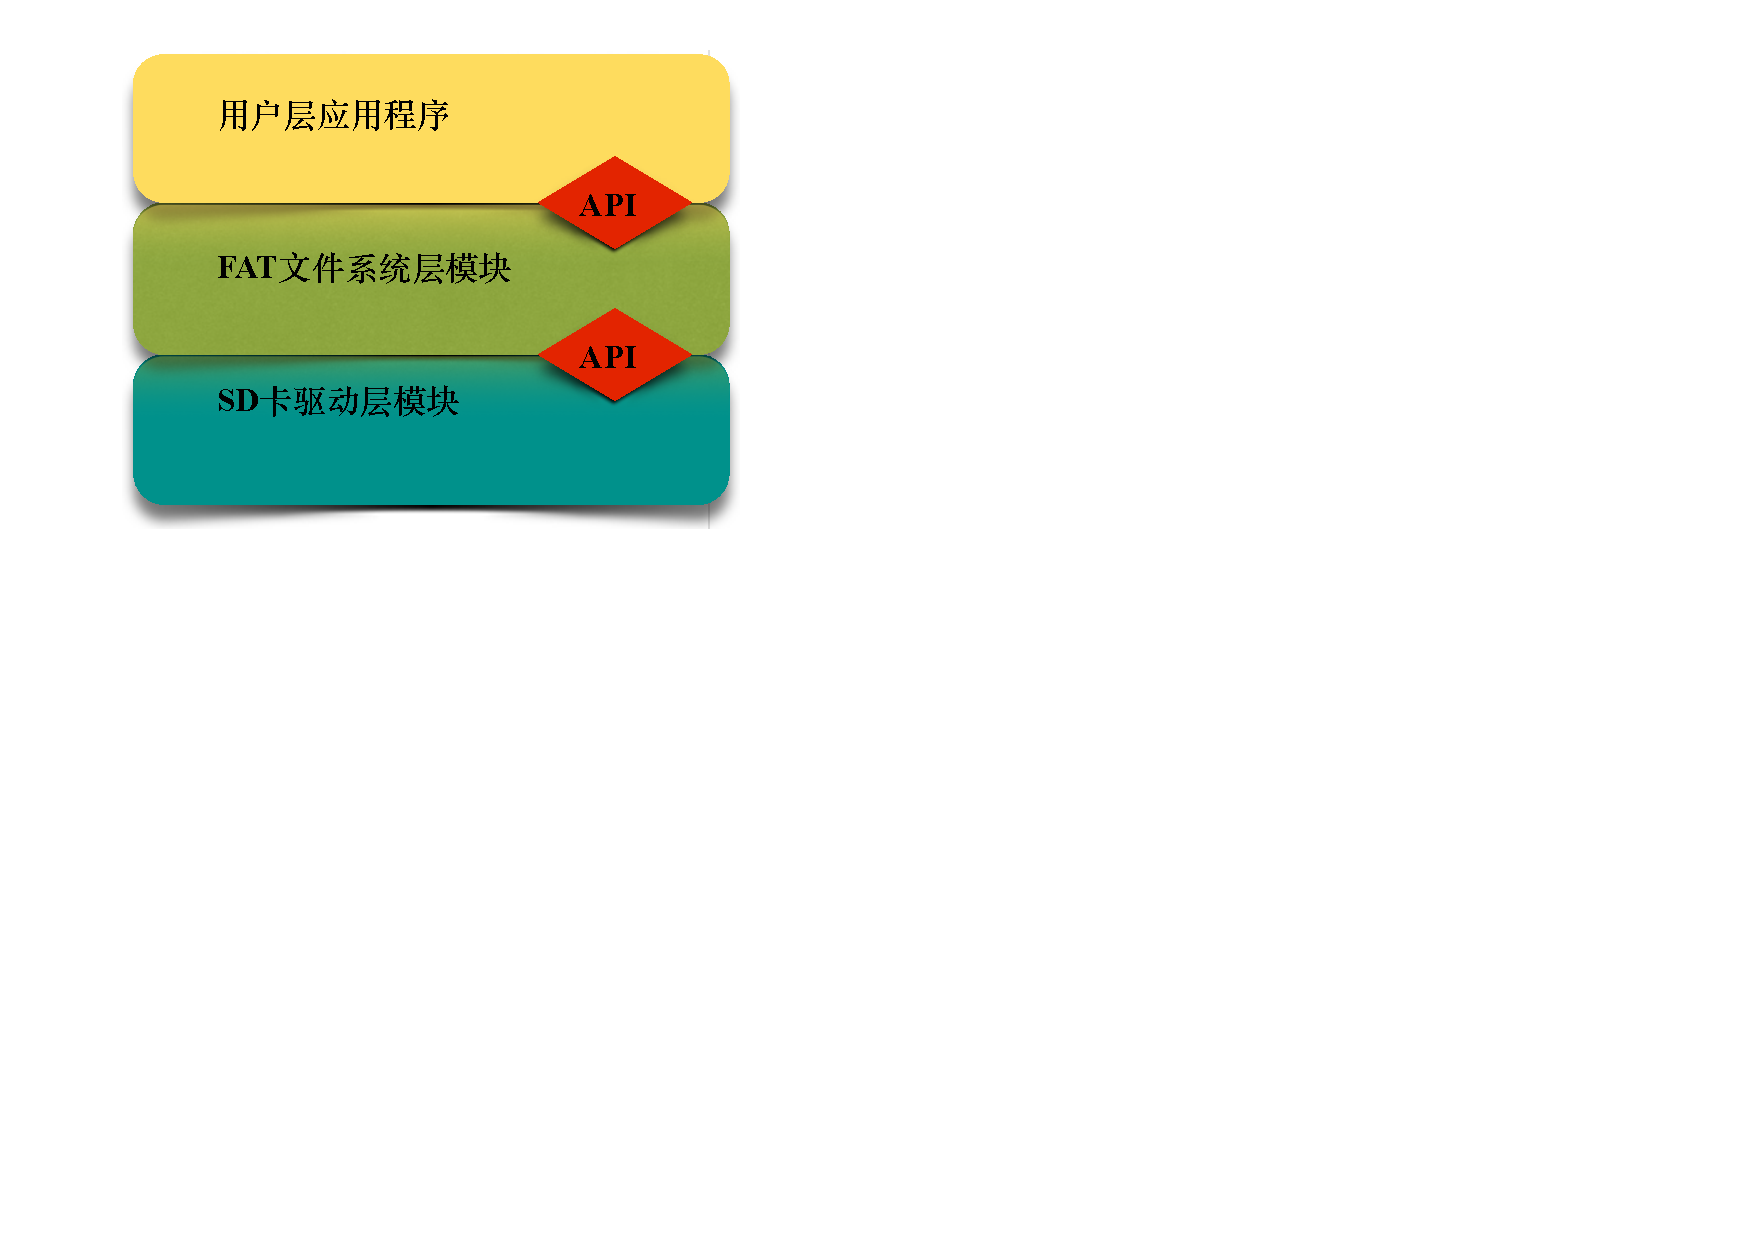
\includegraphics[width=0.5\textwidth]{chap2/layer.pdf}
    \\
    \caption{整体的架构层次}\label{fig:specflow}
\end{figure}

\section{API设计}
\label{sec:API}
通过研究第\ref{sec:Contributions}节的文件系统接口的实际功能和作用,可以完成上层模块的API设计,
该模块的API将为用户的应用程序提供服务,可以被用户程序调用,具体接口如下:
\begin{longtable}[!htb]{ll}
\caption{FAT文件系统模块的API} \label{tab:fatapi}\\
    \toprule
    f\_detect() & SD卡插入检测 \\ \midrule
    f\_mount() & FAT文件系统的挂载\\ \midrule
    f\_open() & 创建新文件或打开文件\\ \midrule
    f\_close() & 关闭文件\\ \midrule
    f\_read() & 从文件读出指定大小的数据到缓存\\ \midrule
    f\_write() & 从缓存写入指定大小的数据到文件\\ \midrule
    f\_seek\_ptr() & 重设文件中的读写指针位置\\ \midrule
    f\_rm() & 删除文件\\
    \bottomrule
\end{longtable}

考虑到FAT模块需要与底层的硬件层通信,本工程在相应的SD卡驱动模块上也留出了API接口,以供FAT模块调用,
FAT模块通过驱动模块实现了数据的物理传输。
\begin{longtable}[!htb]{ll}
\caption{SD卡驱动模块的API} \label{tab:sdapi}\\
    \toprule
    disk\_initialize () & 底层硬件设备的初始化\\ \midrule
    disk\_read () & 读扇区块(512字节)\\ \midrule
    disk\_write () & 写扇区块(512字节)\\ \midrule
    disk\_offset() & 修正逻辑扇区号与物理扇区号的偏移\\
    \bottomrule
\end{longtable}

\section{FAT32文件系统设计}
\label{sec:FAT32}
整个FAT文件系统最初是基于IBM的PC架构而研发的,由此有一个很重要的特性就是,
FAT文件系统在磁盘上的数据是以小端模式\footnote{与此相对的,还存在另一种存储方式,
即大端模式(Big Endian)}(Little Endian)存储的。
\begin{table}[!htb]
  \centering
  \caption[小端模式存储示例]{32位数据在小端模式下的结构}\label{tab:littleendian}
  \begin{tabular}{lcr} \toprule
      byte[3] & &3 3 2 2 2 2 2 2 \\
              & &1 0 9 8 7 6 5 4 \\
      byte[2] & &2 2 2 2 1 1 1 1 \\
              & &3 2 1 0 9 8 7 6 \\
      byte[1] & &1 1 1 1 1 1 0 0 \\
              & &5 4 3 2 1 0 9 8 \\
      byte[0] & &0 0 0 0 0 0 0 0 \\
              & &7 6 5 4 3 2 1 0 \\ \bottomrule
  \end{tabular}
\end{table}

\noindent 一个FAT文件系统卷由四个基本区域组成,它们顺序排列如下:
\begin{enumerate}[noitemsep,topsep=0pt,parsep=0pt,partopsep=0pt,leftmargin=1cm]
    \item[0) ––]
保留区(Reserved Region),磁盘卷上第一个重要的数据结构被称作BPB(BIOS Parameter Block),它位于保留区域(Reserved Region)的第一个扇区。该扇区有时又被称为启动扇区(Boot Sector)或零号扇区($0^{th}$ Sector)。
    \item[1) ––]
FAT表区(FAT Region),文件分配表,是由一些32比特大小的记录项组成的表,它所占据的扇区数目同样在BPB结构用定义,具体位置是「36」字节偏移位置。FAT32通常有FAT数据结构的两份拷贝,这是出于冗余性的考虑。
    \item[2) ––]
根目录区\footnote{FAT32文件系统卷不存在根目录区,相对应地它存在一个动态的根目录表}(Root Directory Region),通常都是将根目录区放在本区域的第一个簇。簇「Cluster」,是由固定数目组成的相邻扇区集群,这个数目在BPB中定义,处于启动扇区的「13」字节偏移位。
    \item[3) ––]
数据区(File and Directory Data Region),包含了磁盘卷剩余的所有扇区,是文件和目录数据真正存储的地方。
\end{enumerate}

FAT表是一张记录了哪些簇号已用、空闲或不可用的表,不仅如此,它还记录了文件的簇链信息。鉴于所使用的FAT文件系统类型不同和磁盘卷的大小不一,一个簇包含的扇区数目可以有多种取值,具体值可以在「BPB」中进行定义。
对于FAT32,尽管FAT表的一条记录项有32位的长度,但只有低28位可用,因此FAT32文件系统可以支援的最大磁盘卷容量是$2^{28} \times 64 \times 512$字节\footnote{此处的「64」为每簇扇区数的最大可用值,「512」为扇区字节数的推荐值},即8TB。

FAT32卷上的每一个文件或目录(根目录除外)都在父目录表上有一条记录,包含着『名称』、『属性』、『大小』以及32位长度的『起始簇号』等信息。
FAT文件系统中的目录,在物理上与文件有相同的组织形式,这种特殊的文件是由一系列32字节的目录记录(Directory Entry)所组成的表,
故目录文件实际上是一张动态的目录表。
FAT32的根目录\footnote{根目录,Root Directory,其起始簇号通常被分配为「2」号簇,故往往是在数据区最开始的扇区簇中。}的与普通目录的不同之处在于,根目录没有时间戳(Date or Time Stamps),没有文件名(只有隐含文件名「\textbackslash」),并且没有「当前目录」(「.」)文件和「父目录」(「..」)文件。另外,根目录还有比较特殊的一点是,它是文件卷上唯一一个可以合法拥有「ATTR\_VOLUME\_ID」标志位的文件。

要完成FAT32文件系统模块的设计,首先要将该模块进一步细分。
在之前的API中,「f\_open()」、「f\_rm()」两个函数需要创建和删除文件,这其中涉及到了对FAT表操作,
最主要的就是新建或者续接簇链(「create\_chain()」)和删除簇链(「remove\_chain()」)。在更新簇链时,
需要对FAT表项进行读取(「get\_fat()」)和更新(「put\_fat()」)。
这两个函数还涉及到了对父目录表的操作,如在目录表上注册一条记录项(「dir\_register()」)、在目录表中寻找指定的记录(「dir\_find()」)、
目录表指针回溯(「dir\_rewind()」)以及指针指向下一条目录项(「dir\_next()」)等。

对「f\_read()」和「f\_write()」函数,如果读写的字节不跨簇的话,不需要与FAT表交互。否则,同样需要通过访问FAT表,遍历文件所在的簇链进行读写。
特别地是,读函数不需要更新FAT表的记录,而写函数有可能会调用「create\_chain()」函数,因为当写入的字节超过已分配的空间时需要向FAT表申请更多的簇来储存数据。

「f\_mount()」函数只需要调用驱动层的初始化函数,之后正确识别并载入「DBR」的启动扇区到内存,最后读取相应的参数信息并使标志位有效即可完成挂载操作。
现在直观地描述如下:

\begin{lstlisting}[basicstyle=\small\ttfamily,caption={FAT文件系统模块结构},label=layout,numbers=none]
├─── f_mount()
├─── f_detect()
├─── f_open()
│       ├────── dir_register()
│       │           ├──────── dir_next()
│       │           ├──────── create_chain()
│       │           │               ├─────── get_fat()
│       │           │               └─────── put_fat()
│       │           └──────── dir_rewind()
│       └────── dir_find()
├─── f_read()
│       └────── getfat()
├─── f_write()
│       ├────── getfat()
│       └────── create_chain()
│                ├──────── get_fat()
│                └──────── put_fat()
├─── f_rm()
│       ├────── dir_find()
│       ├────── get_cluster()
│       └────── remove_chain()
│                ├──────── get_fat()
│                └──────── put_fat()
├─── f_seek_ptr()
└─── f_close()
\end{lstlisting}

上图中的每一次缩进,都表示函数进行了一次调用,对驱动层函数(disk\_read()等)的调用没有画出来。
「f\_detect()」、「f\_close()」等函数相对比较容易实现,对于「f\_open()」、「f\_write()」而言相对复杂一些,
这些函数的具体实现方法将留在\ref{chap:Implementation}详述。

\section{硬件驱动模块的设计}
\label{sec:Driver}
如前所述,SD卡的驱动模块选择了SPI总线协议完成单片机与SD卡的通信,
故在本模块主要需要实现的是由内存向硬件(在本实验中是SD卡)中写入数据以及从中读取数据到内存,
分别由「disk\_read()」和「disk\_write()」实现。鉴于扇区字节数通常都是512字节,并且单片机的内存也是紧俏资源,
故使每次读写的数据块大小都为512字节,即一个扇区。

对于多数磁盘卷,「DBR」扇区往往不是物理扇区第一块,而是由于隐藏扇区的关系有一个偏移值,「disk\_offset()」会完成逻辑扇区号与物理扇区号之间的转换。

\section{小结}
\label{sec:Sum2}
本章具体描述了本工程的整体架构以及各模块预留的应用程序接口,简要剖析了FAT文件系统的设计思路,
描述了FAT模块相关函数的作用功能以及各自的相互调用关系,勾勒出了FAT文件系统模块的大体轮廓,
同时,简要描述了SD卡驱动模块的主要函数和功能,为之后的具体实现做好了理论准备。
